
\chapter{A pipeline for RNA sequencing data analysis}
\label{chapter:methods}
% this should be for general methods 
% within each chapter I can talk about how I used these methods


The workhorse of my PhD is the processing of a large amount of RNA sequencing data, henceforth described as RNA-seq. To do so efficiently and effectively at scale requires a carefully thought out pipeline. Below I describe each section of the analysis pipeline collaboratively developed by the group of Vincent Plagnol but adapted and occasionally broken by myself. The pipeline is optimised for the UCL Computer Science cluster but is freely available to all from \url{github.com/plagnollab/RNASeq_pipeline/}

% insert flowchart of RNA-seq pipeline
\begin{figure}[h!]
	\begin{center}
		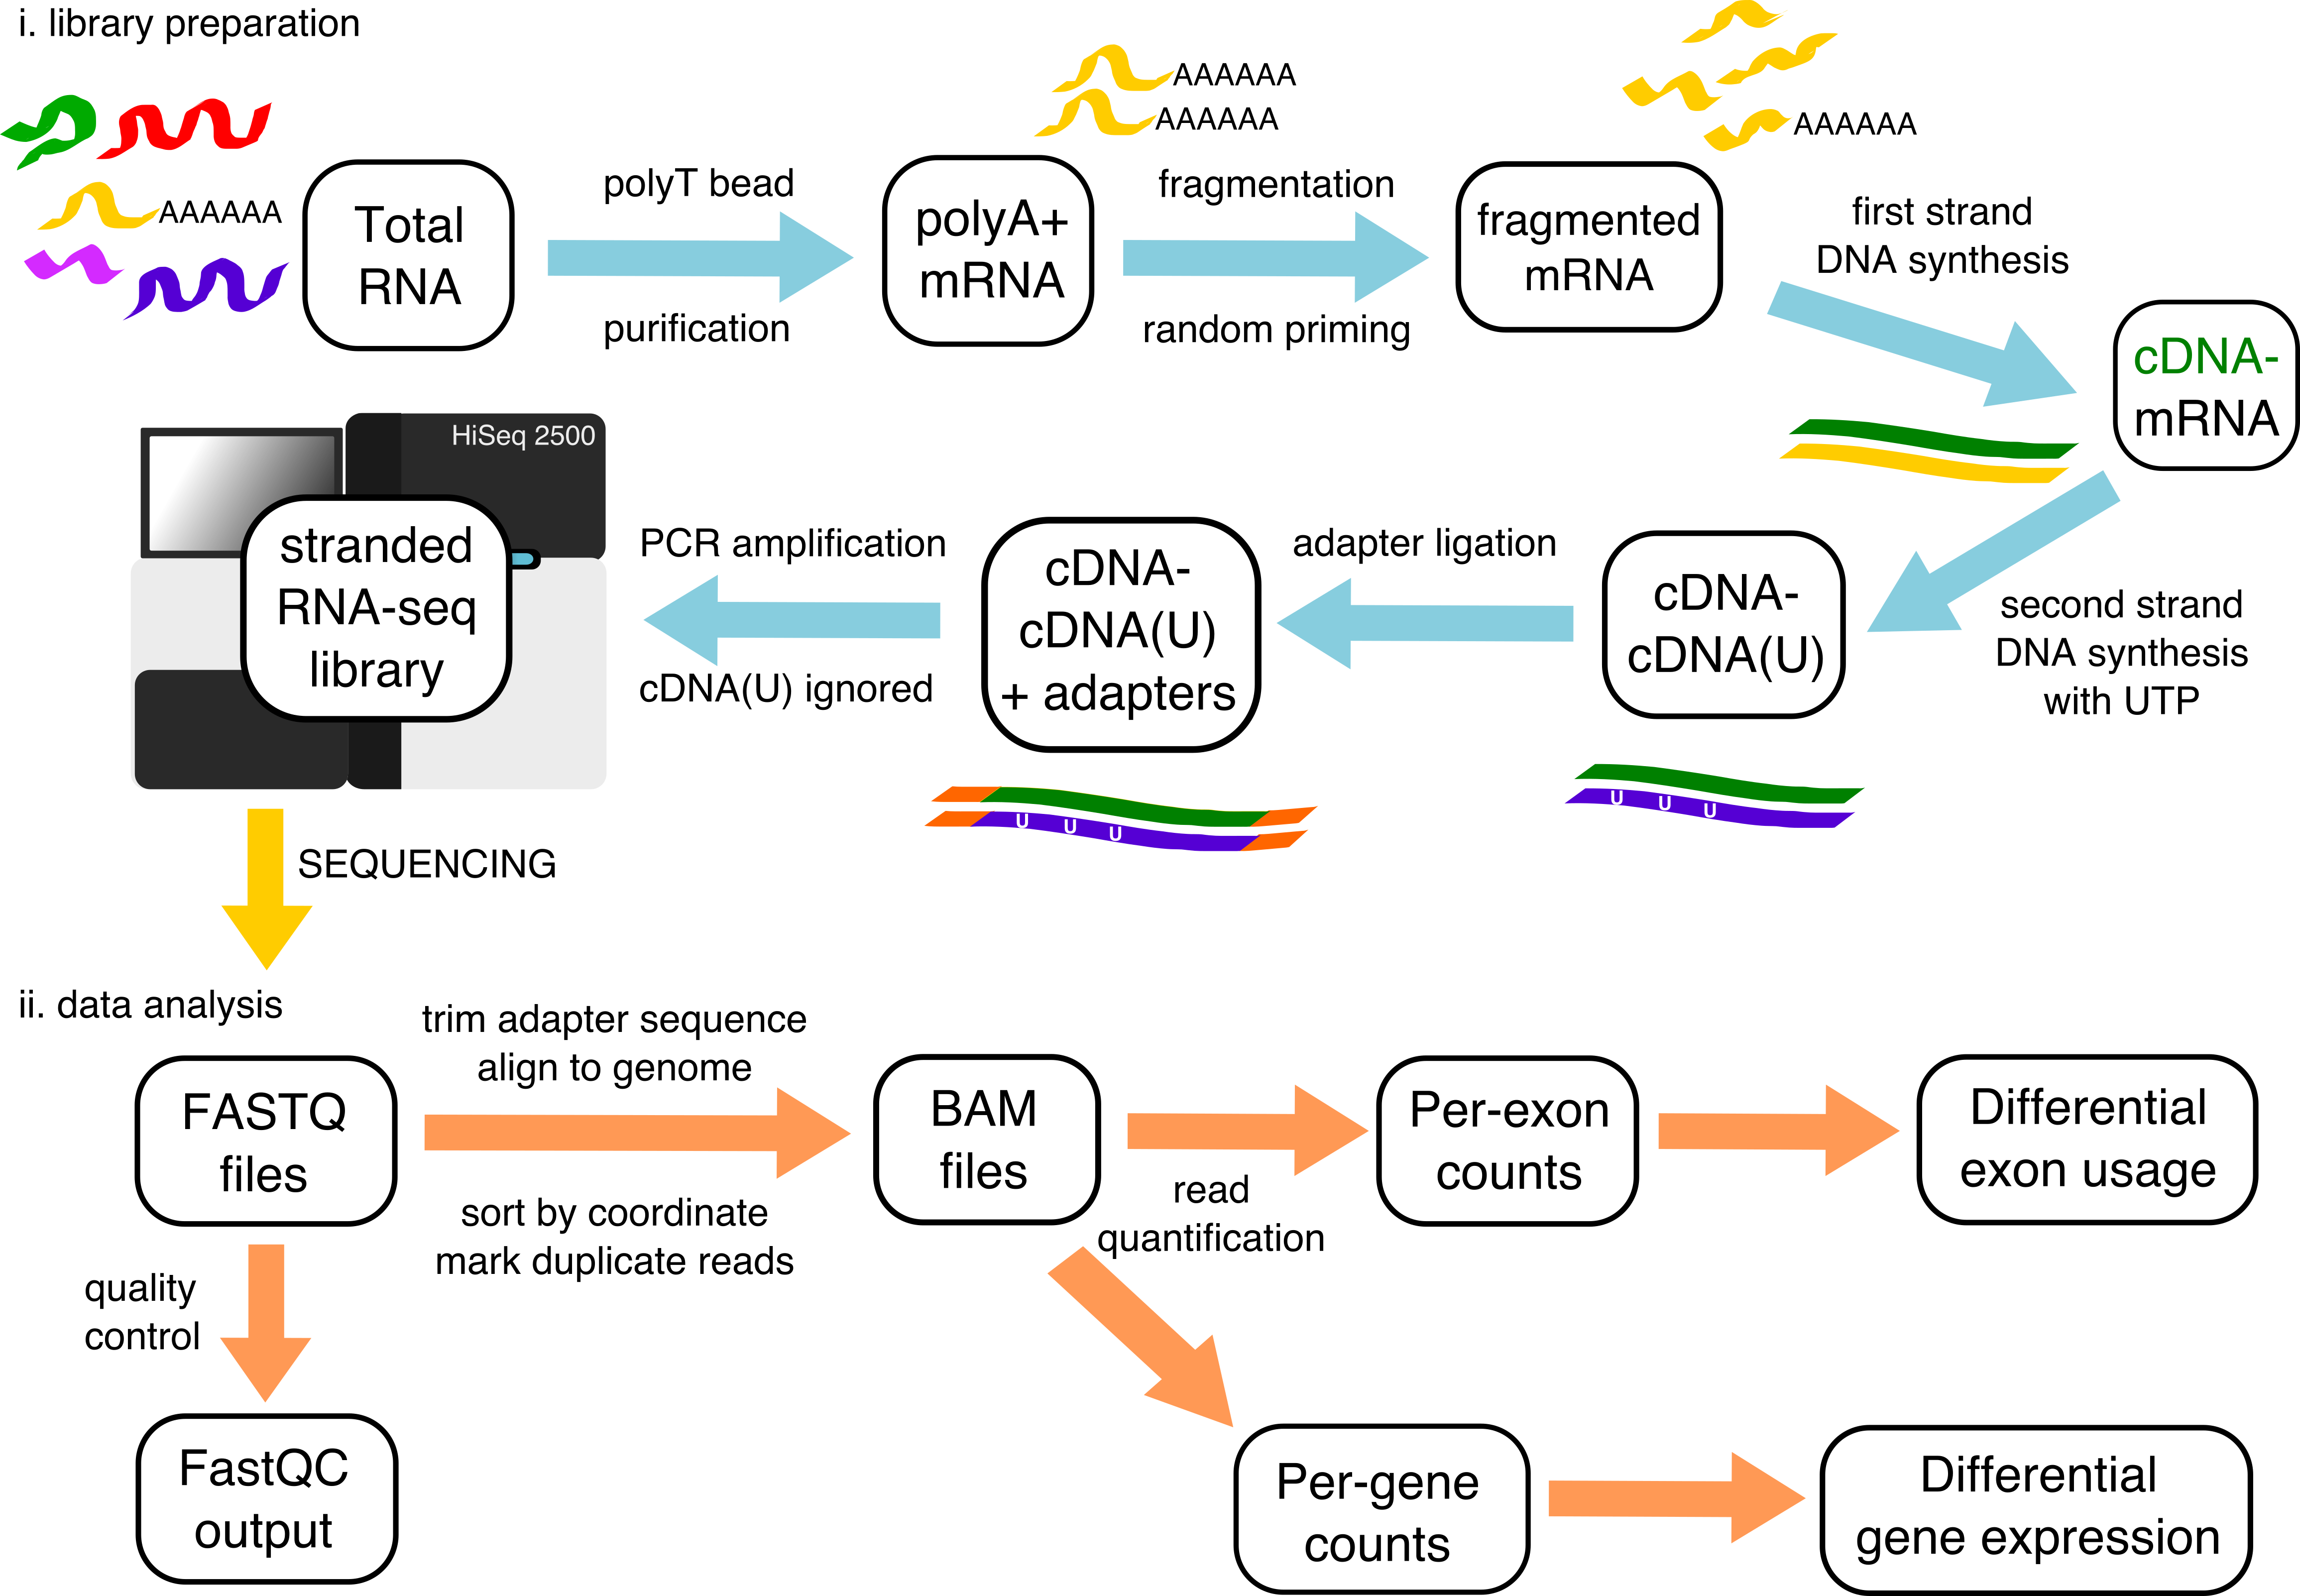
\includegraphics[width=14cm]{Figures/02_methods/RNAseq_pipeline_schematic.png}
	\end{center}
	\caption{Pipeline for stranded RNA-seq preparation and analysis}
	i) Library preparation from total RNA extraction and strand-specific amplification\\
	ii) Bioinformatic analysis workflow to align reads and test for differential gene expression and exon usage
\end{figure}

\section{Library preparation and sequencing}
I feel it is important to understand the preparation of a short read sequencing library so as to best interpret the data in downstream analyses. The description below is of a typical Illumina stranded RNA-seq library preparation.

Briefly, total RNA is extracted from cells or tissues using Trizol or a similar phenol/chloroform reagent \citep{Chomczynski1987}. The majority of RNA species in the cell are ribosomal RNAs. To enrich for mRNA species the RNA is mixed with magnetic beads that are bound to poly(Thymine) oligonucleotides, complementary to the poly(Adenine) tail at the 3' end of mRNA. The RNA is then fragmented. As paired-end sequencing extracts information from each end of the fragment it is important to consider the fragment size in light of the subsequent length of the reads, as with short fragments and long reads the read pairs will overlap leading to redundant information. Pseudo-random barcodes are ligated to each fragment to allow for reverse transcription. The first round of reverse-transcription is carried out forming double stranded DNA-RNA hybrids. These complexes are annealed and a second reverse-transcription reaction is carried out in the presence of Uracil instead of Thymine, creating double stranded DNA. The Uracilated DNA strand is now in the same orientation as the original mRNA fragment. Polymerase chain reaction amplification is then carried out where the uracil containing DNA and the RNA are ignored by the polymerase. The resulting library is strand-specific as all the DNA fragments are antisense to the original RNA fragments. Further adapters are added for sequencing in the flowcell and to give the fragments from each sample an identifier as multiple samples are usually pooled together. 
The standard Illumina paired-end sequencing reaction ligates the amplified fragments to wells in the flowcell which then form clusters of identical amplified fragments. Sequencing then occurs by sequential addition of fluorescent nucleotides along the length of a fragment in both directions, the  colour of which is recorded by a high resolution sensor. The identity of each nucleotide is determined and given a quality score based on the confidence of the measurement. The reads are converted to a FASTQ file, with separate files for the forward and reverse reads. This is a digital encoding of the sequence of both ends of each DNA fragment.

\section{Quality control and read alignment}
The first step in any analysis is quality control of the FASTQ files. Popular tools like \textit{FastQC} (\url{bioinformatics.babraham.ac.uk/projects/fastqc/}) analyse a set of FASTQ files and produce visualisations of multiple diagnostic tests. It can be useful to observe the range of quality scores and how they alter throughout the length of a read to diagnose faults during the sequencing reaction. Another important diagnostic is the presence of adapter sequences within reads. This can occur when the fragmentation step is too aggressive or when the original RNA sample is heavily degraded, often the case in human brain samples. With very short fragments, the sequential addition of nucleotides runs into the adapter sequence of the reads, making these reads much more difficult to align. These universal adapter sequences can be removed by software such as \textit{Trim Galore!} (\url{bioinformatics.babraham.ac.uk/projects/trim_galore/}), which can also remove low quality sequence from the ends of reads, which often occurs towards the end of a sequencing run. 

Following trimming, the FASTQ files must then be aligned to the genome of the species in question. There have been great advancements in speed and accuracy in alignment algorithms, but the key difference between DNA and RNA alignment is the need for read splitting. As most mRNAs are spliced, any RNA fragment that originates from the boundary between two exons will need to be split and both pieces separately aligned to the genome. The interval between two pieces is then recorded by the aligner as a splice junction, the demarcation of where an intron was excised. The current state-of-the-art algorithm in both speed and accuracy at resolving splice junctions is \textit{STAR} \citep{Dobin2013-ra}, which derives its speed from loading the entire genome into memory and then mapping millions of reads per hour using a seed-and-extend algorithm, where small pieces of each read are aligned and incrementally extended to find the best possible split alignment. The alignment information for each read is recorded in a BAM file. Reads from each pair are initially recorded next to each other and the BAM file is ordered by the read name. However for most downstream analyses the BAM file must be re-ordered by genomic position. Our pipeline does this using the \textit{Novosort} algorithm (\url{http://www.novocraft.com/products/novosort/}). 

Another potential issue in RNA-seq data, particularly in older data or from human brain-derived RNA, is a bias towards fragments from the 3' end of mRNAs. This can also occur due to mRNA degradation before the poly(Thymine) purification which will then bias the library to sequences closest to the bound polyadenylation site at the 3' end. This can be obvious when observing coverage across all genes with a diagnostic package such as \textit{QoRTS} \citep{Hartley2015a}. As most differential expression software assumes even coverage throughout a gene body, heavily degraded samples can skew the estimates of gene or exon expression.

For downstream expression analysis, the aligned reads are then quantified for a set of features. These features can either can be whole genes or individual exons. There are multiple annotations for the human and mouse genome for where the known genes and exons are but our pipeline uses the Ensembl transcript annotation as our reference \citep{Cunningham2015}. Reads that overlap each gene or individual exon are counted using \textit{HTSeq} \citep{Anders2015-wz}.


\section{Differential gene expression}
The most common application of RNA-seq is for an experiment comparing the abundances of different RNAs between conditions, for example between the knockdown of a particular gene and a control. These experiments should be made up of multiple biological replicates, where RNA libraries have been prepared from different organisms or cell culture samples under the same conditions. This is so a fair assessment can be made of the biological variation in RNA abundance within each condition. This is in comparison to technical replicates, where the same library is sequenced multiple times, which only tells you about the variance in the measurement. The still-expensive cost of sequencing usually limits a lab to sequence a small number of biological replicates, which limits one's statistical power to detect small variations in RNA abundance and the confidence in the truth of one's results. There are multiple algorithms to test for differential expression but we have settled on using the \textit{DESeq2} package for its statistical robustness and speed \citep{Love2014}.
Differential expression algorithms attempt to compensate for the small sample sizes by making use of the fact that each sequencing library measures the abundance of tens of thousands of genes. The number of reads generated by each library can be highly variable and so this is also accounted for. \textit{DESeq2} normalises the read counts for each gene in each sample by the size of each sample's library, a \textit{size factor}. It then assumes that the normalised read counts fit a negative binomial probability distribution. It then estimates the variance or dispersion in read count for each gene across the samples. To compensate for small sample sizes, which tend to give a very high estimate of dispersion, it compares the dispersion between all genes and shrinks the estimate to a local average dispersion based on genes expressed at a similar level. Using these shrunken dispersion estimates, the software then fits two generalised linear models: a null model where condition has no effect and an alternative model where the change in condition explains the change in gene expression. The two models are compared with a Wald test on which model fits the data better, computing a P-value. The P-values generated for each gene are adjusted to correct for multiple testing using the Benjamini-Hochberg procedure \citep{Benjamini1995}. The output of a differential expression analysis gives you both an adjusted P value for each gene and a $log_2$ of the fold change in expression between the two conditions to give you an estimate of the effect size. A positive fold change indicates an increase in the treatment versus the control. 

%%\section{Gene ontology analysis } % only keep in if I have to write up Anny's work
%%Using GOSeq to correct for length bias in RNA-seq gene ontology 

\section{Quantifying annotated splicing changes }
Following differential gene expression analysis, the next most popular use for RNA-seq is in understanding changes in splicing across conditions. This can be tackled with multiple approaches but one of the most widely used methods is differential exon usage analysis, which was made available by the \textit{DEXSeq} package \citep{Anders2012}. Rather than measuring the abundance of individual isoforms, \textit{DEXSeq} requires a flattened list of "union exons" which is a set of non-overlapping intervals for each exon from each annotated transcript in a given gene. RNA-seq seq reads can then be counted at each union exon. \textit{DEXSeq} then compares the \textit{size factor} normalised counts from each exon with the counts from all the exons in a gene and how they vary across biological conditions, again with the use of generalised linear model. 
The output of a \textit{DEXSeq} analysis is each union exon in a gene is given a $log_2$ fold change between conditions and an adjusted P value from the test. Although this output can be used to demonstrate whether differential exon usage occurs due a condition, it is inherently difficult to extract meaningful information about the underlying biology. A significant union exon may not correspond to real exon. Therefore, hits from \textit{DEXSeq} need to be closely analysed in the context of the gene they reside in. Chapter 5 discusses recent alternatives to \textit{DEXSeq}. 


